\subsection{Test-System}
Wie bereits erw�hnt werden im Test-System die 889 angebotenen Interfaces verwendet, die auch im Hei�-System verwendet werden. Dar�ber hinaus wurden noch 6 weitere angebotene Interfaces dem Test-System hinzugef�gt, um bestimmte Konstellationen geziel zu evaluieren. Die 6 erwarteten Interfaces wurden wie folgt deklariert (siehe \abbsrefs{tei1}{tei6}).


\myBigFigure{ElerFTFoerderprogrammeProvider}{Erwartetes Interface: ElerFTFoerderprogrammeProvider}{tei1}
\myBigFigure{FoerderprogrammeProvider}{Erwartetes Interface: FoerderprogrammeProvider}{tei2}


\begin{figure}[H]
\begin{minipage}[b]{.57\linewidth}
%\begin{flushleft}
  \centering
  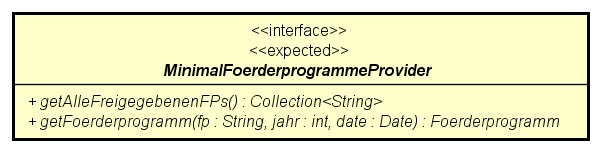
\includegraphics[width=\linewidth]{MinimalFoerderprogrammeProvider}
  \caption{Erwartetes Interface: MinimalFoerderprogrammeProvider}
  \label{abb:tei3}

%\end{flushleft}
\end{minipage}%
\hspace{.03\linewidth}% Abstand zwischen Bilder
\begin{minipage}[b]{.4\linewidth}
%\begin{flushright}

  \centering
  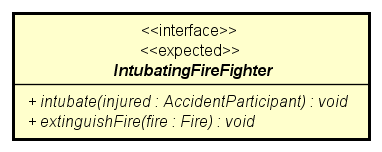
\includegraphics[width=\linewidth]{IntubatingFireFighter}
  \caption{Erwartetes Interface: IntubatingFireFighter}
  \label{abb:tei4}

%\end{flushright}
\end{minipage}
\end{figure}



\begin{multicols}{2}
\myBigFigure[8cm]{IntubatingFreeing}{Erwartetes Interface: IntubatingFreeing}{tei5}
\myBigFigure[8cm]{IntubatingPatientFireFighter}{Erwartetes Interface: IntubatingPatientFireFighter}{tei6}
\end{multicols}
\newpage
\noindent
Im weiteren Verlauf werden die oben beschriebenen Interfaces durch die K�rzel in \tabref{eIShort} identifiziert.
\begin{table}[H]
\centering
\small
\begin{tabular}{|l|c|}
\hline
\hline
\centering\textbf{erwartetes Inferface} & \textbf{K�rzel} \\
\hline
\hline
ElerFTFoerderprogrammeProvider & TEI1\\
\hline
FoerderprogrammeProvider & TEI2\\
\hline
MinimalFoerderprogrammeProvider & TEI3\\
\hline
IntubatingFireFighter & TEI4\\
\hline
IntubatingFreeing & TEI5\\
\hline
IntubatingPatientFireFighter & TEI6\\
\hline
\hline
\end{tabular}
\caption{K�rzel der erwarteten Interfaces}
 \label{tab:eIShort}
\end{table}


\section{Ergebnisse für die Heuristik LMF}\label{sec_evalLMF}
In Bezug auf die Heuristik \emph{LMF} gilt es nicht nur zu evaluieren, ob die Suche nach einem Proxy, der die vordefinierten Tests besteht, beschleunigt werden kann, sondern auch, mit welcher Variante zur Bestimmung des Matcherratings (vgl. Abschnitt \ref{sec_lmf}) die besten Ergebnisse erzielt werden können. 
\\\\
Hierzu wird die Exploration für alle der oben genannten \emph{required Typen} für jede Variante zur Bestimmung der Matcherratings durchgeführt (siehe Abschnitt \ref{sec_lmf} Tabelle \ref{tab_matcherratingvarianten}). Im folgenden Verlauf wird lediglich auf die Variante eingegangen, die die besten Ergebnisse hervorgebracht hat. Die Ergebnisse unter Verwendung der übrigen Varianten sind im Anhang \ref{app_matcherratingEval} zu finden.
\\\\
Die Variante \emph{1.1} (vgl. Tabelle \ref{tab_matcherratingvarianten}) erbrachte die besten Ergebnisse. Die folgenden Vier-Felder-Tafeln zeigen die Ergebnisse mit dieser Variante zur Bestimmung der Matcherratings für die \emph{required Typen} \emph{TEI1}-\emph{TEI3} auf.
\begin{multicols}{3}
\vft{1}{5}{$p(44)-6$}{1}{0}{Ergebnisse \emph{LMF} mit Variante 1.1 für TEI1 \\1. Durchlauf}{lmf11_TEI1_1}
\vft{1}{1889}{$p(55)-1890$}{1}{0}{Ergebnisse \emph{LMF} mit Variante 1.1 für TEI2 1.~\mbox{Durchlauf}}{lmf11_TEI2_1}
\vft{1}{1463}{$p(50)-1464$}{1}{0}{Ergebnisse \emph{LMF} mit Variante 1.1 für TEI3 1.~\mbox{Durchlauf}}{lmf11_TEI3_1}
\end{multicols}
\noindent
Die Ergebnisse für die \emph{required Typen} \emph{TEI4}-\emph{TEI7} zeigen die folgenden Vier-Felder-Tafeln. 
\begin{multicols}{2}
\vft{1}{$1174$}{0}{0}{0}{Ergebnisse \emph{LMF} mit Variante 1.1 für TEI4 1.~\mbox{Durchlauf}}{lmf11_TEI4_1}
\vft{2}{2}{$p(2247)-3$}{1}{0}{Ergebnisse \emph{LMF} mit Variante 1.1 für TEI4 2.~\mbox{Durchlauf}}{lmf11_TEI4_2}
\end{multicols}

\begin{multicols}{2}
\vft{1}{$4984$}{0}{0}{0}{Ergebnisse \emph{LMF} mit Variante 1.1 für TEI5 1.~\mbox{Durchlauf}}{lmf11_TEI5_1}
\vft{2}{32}{$p(2775)-33$}{1}{0}{Ergebnisse \emph{LMF} mit Variante 1.1 für TEI5 2.~\mbox{Durchlauf}}{lmf11_TEI5_2}
\end{multicols}

\begin{multicols}{2}
\vft{1}{$1051$}{0}{0}{0}{Ergebnisse \emph{LMF} mit Variante 1.1 für TEI6 1.~\mbox{Durchlauf}}{lmf11_TEI6_1}
\vft{2}{0}{$p(1323)-1$}{1}{0}{Ergebnisse \emph{LMF} mit Variante 1.1 für TEI6 2.~\mbox{Durchlauf}}{lmf11_TEI6_2}
\end{multicols}

\begin{multicols}{2}
\vft{1}{$161294$}{0}{0}{0}{Ergebnisse \emph{LMF} mit Variante 1.1 für TEI7 1.~\mbox{Durchlauf}}{lmf11_TEI7_1}
\vft{2}{7641}{$p(52150)-7642$}{1}{0}{Ergebnisse \emph{LMF} mit Variante 1.1 für TEI7 2.~\mbox{Durchlauf}}{lmf11_TEI7_2}
\end{multicols}
\noindent
Folgendes kann aus diesen Ergebnissen abgeleitet werden:
\begin{enumerate}
\item Die Heuristik \emph{LMF} erzielt eine Reduktion der zu erzeugenden Proxies. Dies wird durch einen Vergleich der Spalte ``positiv'' innerhalb der Vier-Felder-Tafeln zum jeweiligen \emph{required Typ} belegt.

\item Die Heuristik \emph{LMF} hat keine Auswirkung auf einen Durchlauf, in dem kein Proxy erzeugt wird, mit dem die semantischen Tests erfolgreich durchgeführt werden können. Dies kann durch einen Vergleich des ersten Durchlaufs für die \emph{required Typen} \emph{TEI4}-\emph{TEI7} im Ausgangspunkt (Tabellen \ref{tab:tmr_start_tei4_1}, \ref{tab:tmr_start_tei5_1}, \ref{tab:tmr_start_tei6_1} und \ref{tab:tmr_start_tei6_1}) mit dem ersten Durchlauf unter Anwendung der Heuristik (Tabellen \ref{tab:lmf11_TEI4_1}, \ref{tab:lmf11_TEI5_1}, \ref{tab:lmf11_TEI6_1} und \ref{tab:lmf11_TEI7_1}) festgestellt werden.
\end{enumerate}



%Aus diesen Ergebnissen lässt sich folgendes ableiten:
%\begin{enumerate}
%\item Das Akkumulationsverfahren Nummer 3. (Minimum) führt sowohl für die Typ- und Methoden-Konvertierungsvarianten zu schlechteren Ergebnissen als die anderen drei Akkumulationsverfahren. Es sollte daher für die Heuristik TMR\_Quant nicht verwendet werden.
%\item Die Ergebnisse von 1-2 und 3-2 unterscheiden sich nur geringfügig, obwohl bei 3-2 das Akkumulationsverfahren Nummer 3. zum Einsatz kam. Dies konnte auch bei anderen Kombinationen festgestellt werden, bei denen das 3. Akkumulationsverfahren für die Akkumulation des Type-Matcher Ratings der Typ-Konvertierungsvariante verwendet wurde. Das lässt vermuten, dass die Beachtung des Type-Matcher Ratings einer ganzen Typ-Konvertierungsvariante weitgehend unerheblich für die Heuristik TMR\_Quant ist.
%, wenn das Type-Matcher Rating je Methoden-Konvertierungsvarianten über ein entsprechend gutes Akkumulationsverfahren ermittelt wurde. 
%Dies ist jedoch darauf zurückzuführen, dass das Type-Matcher Rating je Methoden-Konvertierungsvariante die Parameter für die Ermittlung des Type-Matcher Ratings einer Typ-Konvertierungsvariante darstellen.
%\item An den Ergebnissen zu den erwarteten Interfaces TEI4-TEI6 ist zu erkennen, dass die Heuristik TMR\_Quant keinen Einfluss auf den 1. Durchlauf hat. Daraus kann geschlussfolgert werden, dass die Heuristik nur in dem Durchlauf einen Gewinn bringt, in dem auch eine passende benötigte Komponente gefunden werden kann. 
%\end{enumerate}
%Aufgrund der Ergebnisse stehen für die weitere Verwendung der Heuristik TMR\_Qual mehrere Kombinationen von Akkumulationsverfahren zur Auswahl. Die Entscheidung fällt aufgrund der etwas geringeren Komplexität auf die Kombination 1-2. 
